\section{Engine}

\subsection{Overview}

\nomenclature{DOHC}{Dual Overhead Camshafts}

The Formula 2010 vehicle uses a stock \emph{Honda CBR600F4i} motorcycle engine, as pictured in Fig. \ref{fig:cbr600f4i_engine}. It is a \unit{600}{\centi\cubic\metre} super-sport class engine with an internal 6-speed chain driven transmission. The engine utilizes an inline four cylinder configuration. The engine also has \emph{Dual Overhead Camshafts} (DOHC) to allow for four valves per cylinder: two for intake and two for exhaust.

The engine is connected to an \emph{intake system} that directs air to the cylinders and an \emph{engine control unit} for regulating the combustion timing of the engine. The rules for the Formula SAE competitions forbid \emph{drive-by-wire}, meaning that throttle control must be purely mechanical \cite{2010fsaerules}.

\begin{figure}[H]
	\centering
	 	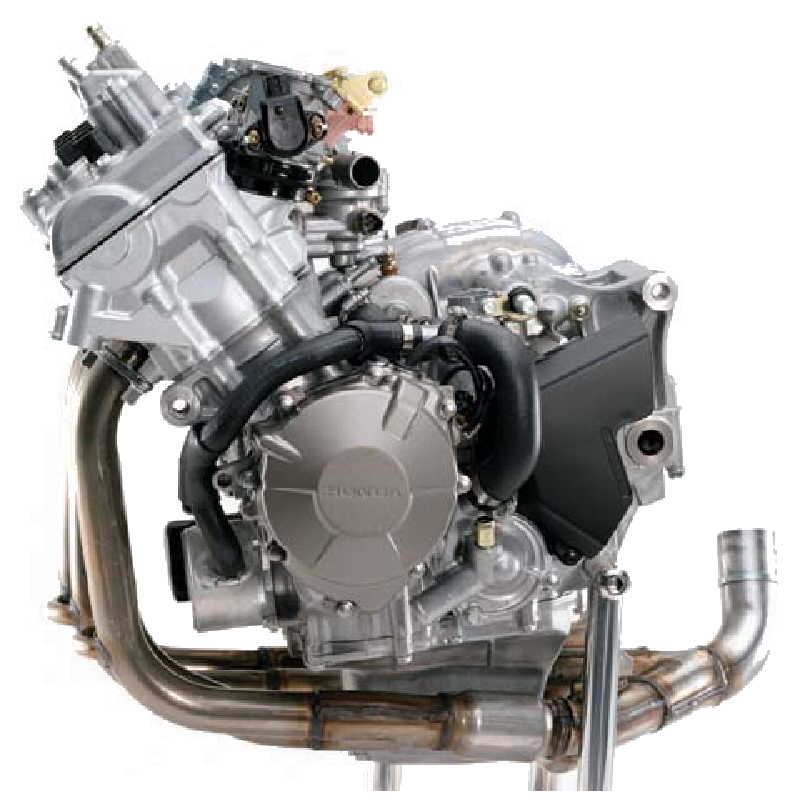
\includegraphics[scale=0.5]{background/figures/cbr600f4i_engine.eps}
    \caption{The Honda CBR600F4i engine.}
    \label{fig:cbr600f4i_engine}
\end{figure}

\subsection{Intake System}

The intake system consists of several parts, including the \emph{throttle-body}, \emph{restrictor}, \emph{intake plenum}, \emph{intake runners}, and \emph{intake valves}. The throttle-body is a valve that controls the amount of air entering the intake system. It is followed by a restrictor, which restricts the maximum air flow into the engine. Use of a restrictor is mandated Formula SAE rules. After the restrictor, the air flows into a large intake plenum. From the plenum, four intake runners lead to each cylinder head, where the intake valves are located.

As the intake valves on the engine open, they generate negative pressure waves that travel the length of the intake runners and back into the intake plenum. There, they reflect and travel back towards the intake valve. This reflection towards the intake valves can act to increase pressure at the valve and increase power.

\nomenclature{RPM}{Revolutions per Minute}

A fair amount of research has been done in previous years on the intake and exhaust design for the Formula SAE car. Former UMSAE engine section head Lucas Groening wrote an undergraduate thesis on modelling of the engine package for the 2008 Formula car. One important dynamic aspect of the engine design that he describes is the effect of the intake runner length on the torque output of the engine at different \emph{Revolutions Per Minute} (RPM) \cite{LucasIntake}. 

Figure \ref{fig:irl_effect} shows a comparison between various intake runner lengths and torque output over the RPM operating range of the engine. Different plenum lengths cause the two torque peaks to occur at different RPMs. Groening proposed that an electronic means of modulating the length of the runners to maximize engine torque could dramatically improve engine performance \cite{LucasIntake}.

\begin{figure}[H]
	\centering
	 	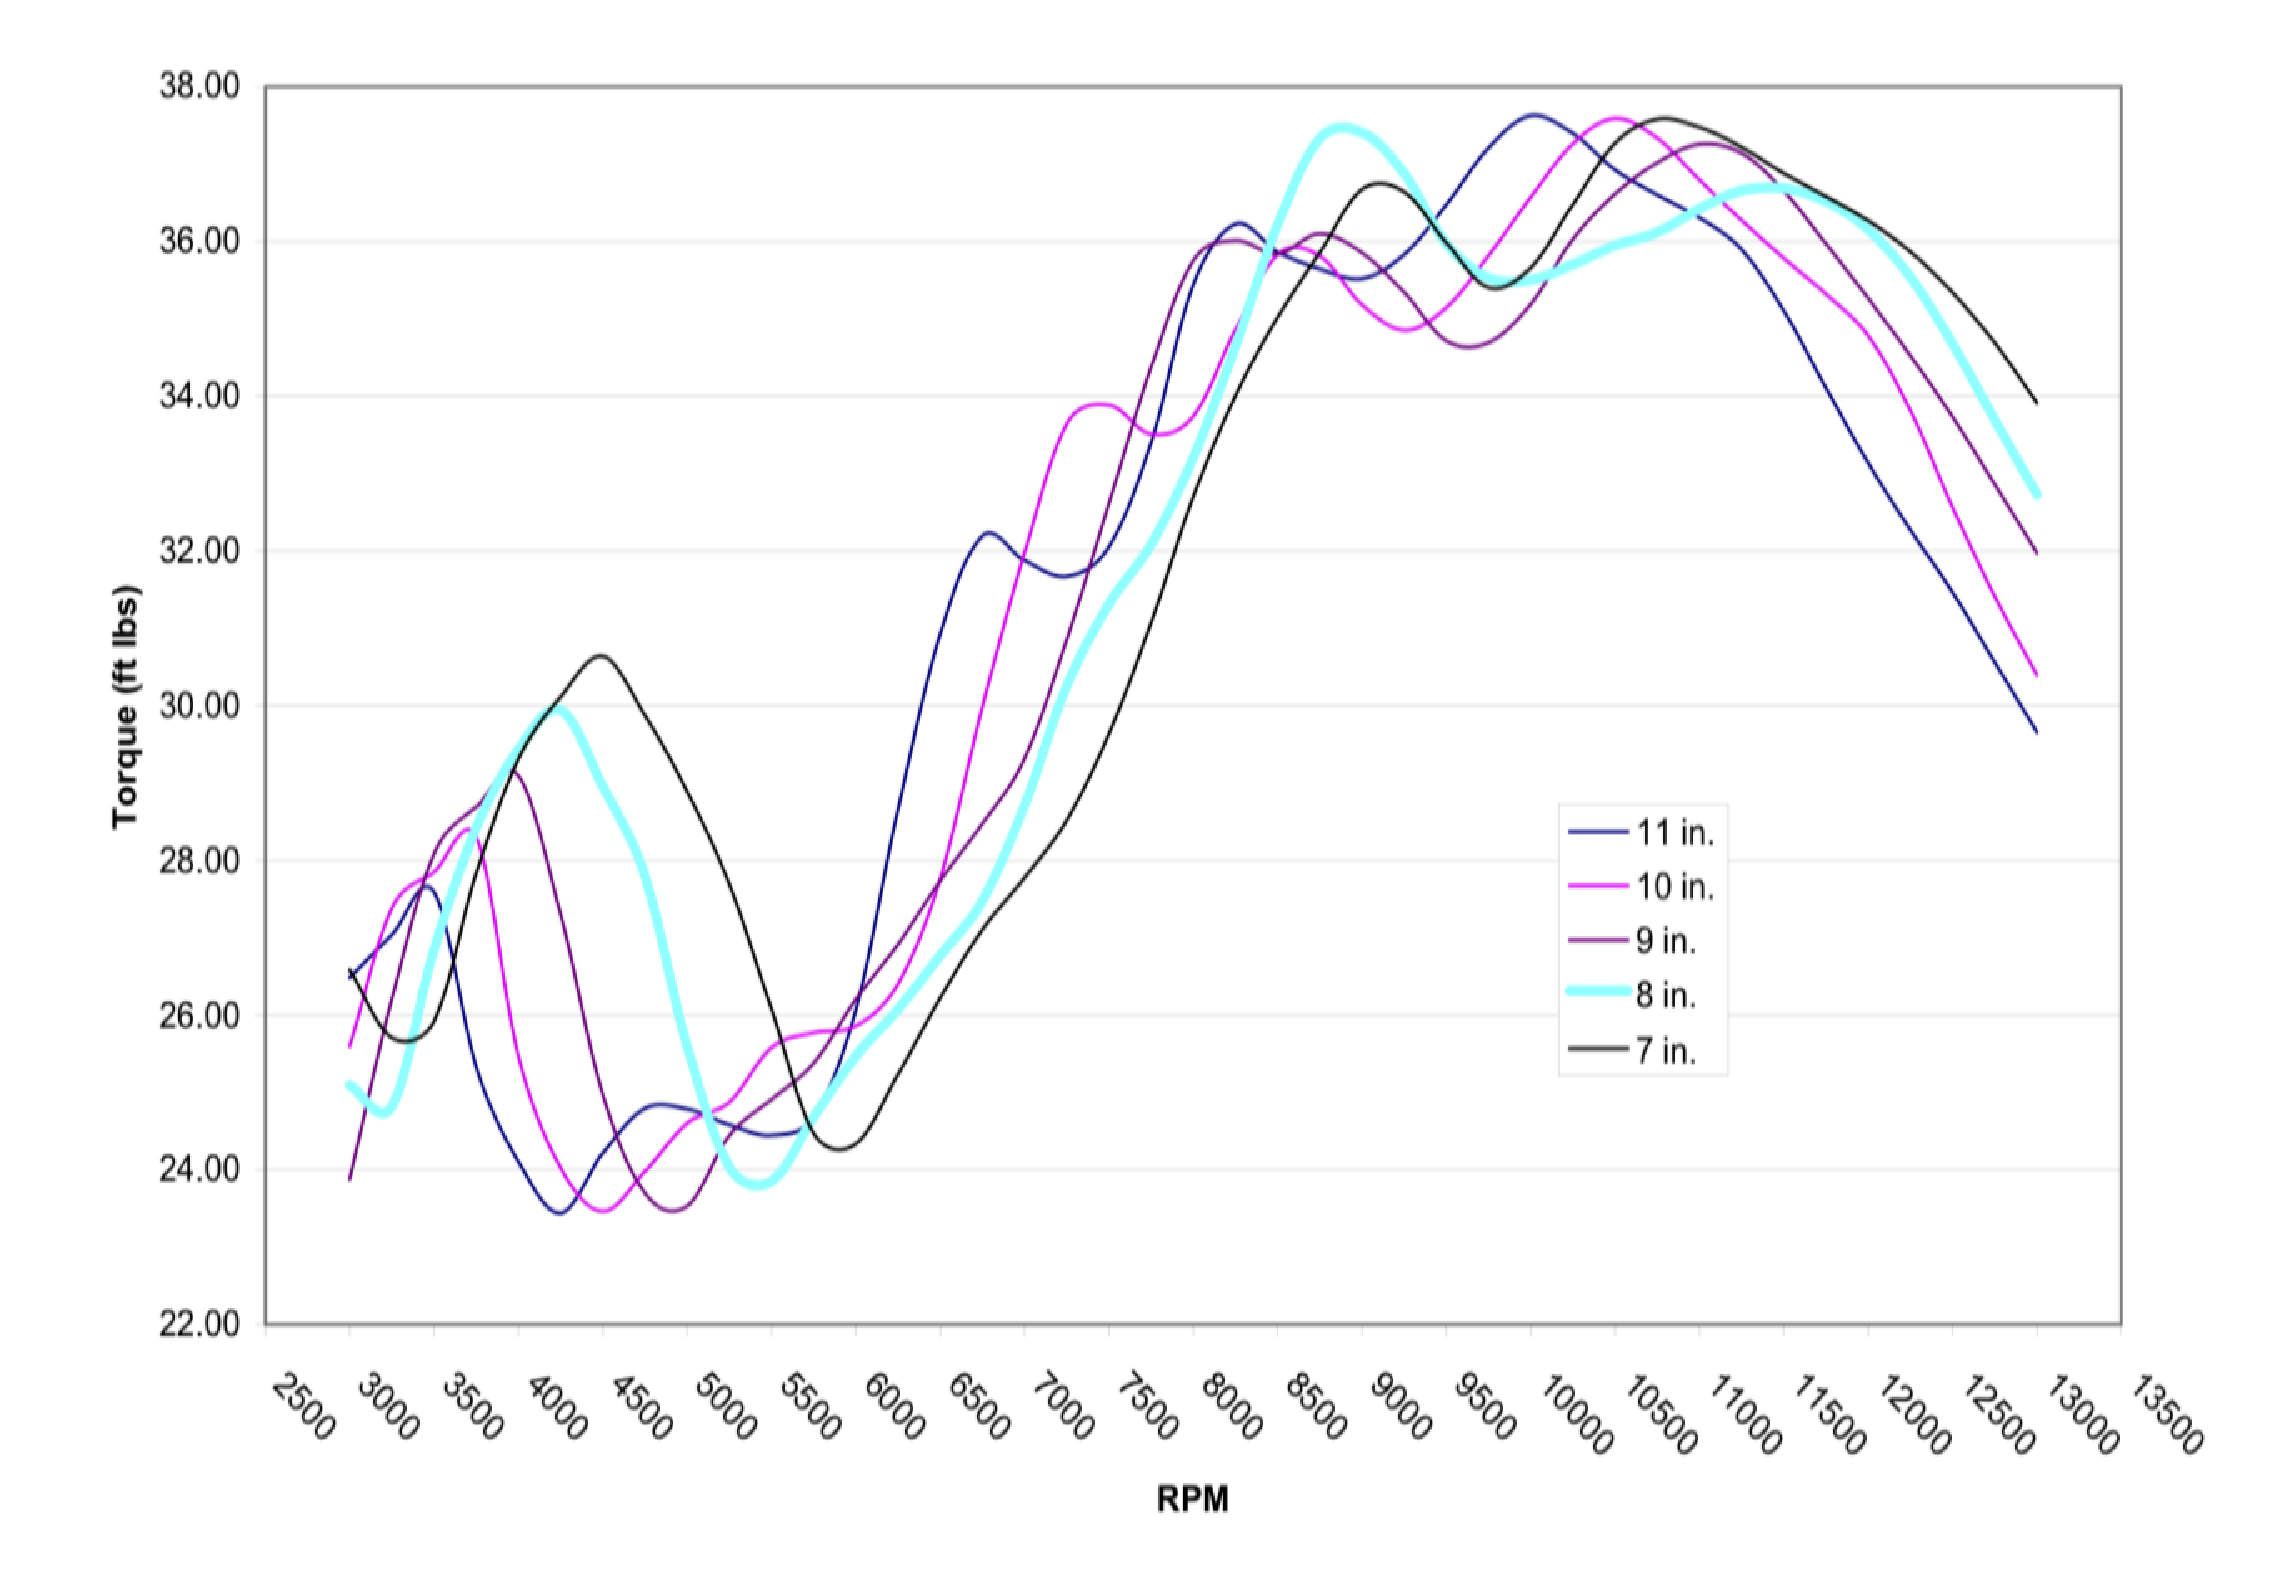
\includegraphics[scale=0.35]{background/figures/irl_effect.eps}
    \caption{The effect of intake runner length on torque for various RPM.}
    \label{fig:irl_effect}
\end{figure}

\subsection{Engine Control Unit}
\label{sec:ECU}

\nomenclature{ECU}{Engine Control Unit}
\nomenclature{MAP}{Manifold Absolute Pressure}

A specialized third-party component called the \emph{Engine Control Unit} (ECU) controls the fuel injector and spark coil systems that in turn control the combustion cycle of the engine. The particular model of ECU used by the Formula SAE car is the S80Pro from DTAFast \cite{s80pro}, as seen in Fig. \ref{fig:s80pro_product}.

\begin{figure}[H]
	\centering
		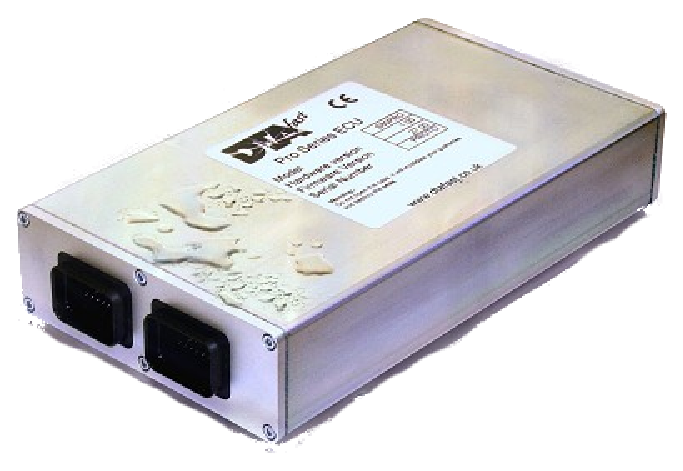
\includegraphics[scale=0.5]{background/figures/s80.eps}
	\caption{The DTAFast S80Pro engine control unit.}
	\label{fig:s80pro_product}
\end{figure}

The ECU uses several sensors to adjust the fuel injector and spark coil timings, such as an \emph{oxygen sensor} to determine the air-to-fuel ratio in the engine, and a \emph{Manifold Absolute Pressure} (MAP) sensor to determine the engine's air mass flow rate. This keeps the engine running smoothly and ensures maximum efficiency and power generation. 

The ECU features a traction control system that monitors wheel slip and cuts spark and fuel to provide traction when one of the wheels is slipping. The ECU also collects the various sensor readings and makes them available to other electronic devices at a fixed frequency through a shared data bus. 

\nomenclature{RS-232}{Recommended Standard 232 for Byte-Oriented Communications}
\nomenclature{CAN}{Controller Area Network}

The ECU communicates with proprietary software on a Windows-based computer over an RS-232 link. The communication protocol used is undocumented and possibly encrypted. The ECU also broadcasts select sensor readings such as engine RPM over a \emph{Controller Area Network} (CAN) interface at a fixed frequency of 10 Hz. The CAN message format is documented in Appendix \ref{cha:ecu_can_spec}.

As well as the aforementioned bus-based interfaces, the ECU provides several CMOS-level discrete outputs:

\begin{itemize}
	\item Launch Control Enable, which allows the ECU to balance power distribution during accelleration;
    \item Shift Cut, which signals the ECU to reduce engine power before a downshift;
    \item Traction Control Enable, which reduces power output when the wheels begin to slip; and
    \item Wet/Dry Selection, which switches between two different sets of traction control parameters.
\end{itemize}

Detailed descriptions of the launch control, shift cut, and traction control features can be found in the S80 user manual \cite{s80pro}.


